\documentclass{article}

\usepackage{graphicx}

\begin{document}

\title{Evolving Random Graph Generating Algorithms}

\author{
Pope, Aaron\\
\texttt{aaron.pope@mst.edu}
\and
Martin, Matthew\\
\texttt{mam446@mst.edu}
}

\maketitle

\section{Introduction}

\subsection{Random Graphs}

Random graphs have a variety of applications in graph theory. The graphs themselves can be described as a model consisting of a probability distribution of degrees, adjacency or some other characteristic. Alternatively, random graphs can be described by a stochastic process of generating a graph within certain constraints. The research presented in this work will focus on this latter approach.

How well a random graph model describes a given graph can be determined by performing a statistical goodness of fit test. Inversely, if a random process is to produce graphs which fit well with a given random graph model, a goodness of fit test performed on a population of resulting graphs with respect to the desired model can be used to determine how well the process produces graphs described by the model. 

It is possible to have desirable features within a graph that are not captured or guaranteed by a random graph model. An example of this would be the occurrence of certain topology motifs within the graph. The presence of these motifs can have a large impact on characteristics of the graph as a whole, such as the resilience or robustness of the graph. These motifs, along with other features, can be detected in the graphs which are generated by a given process. The quality of the graph generating process can be determined by how consistently it produces graphs with a high occurrence of desirable features and a low occurrence of undesirable features.

\subsection{Evolutionary Computing and Genetic Programming}

Evolutionary Computing (EC) uses a biologically inspired process to solve a problem by generating a population of potential solutions and selecting the best among them to participate in procreation to create more solutions. This process continues through multiple generations until certain termination criteria are met. Genetic Programming (GP) is a field of EC in which the solutions sought are programs themselves. The candidate programs can be represented as parse trees in which the internal nodes represent operations on the input received from the children nodes and the leaf nodes are chosen from the problem's input.

Traditional GP has several stochastic components. The population is initialized with randomly created solutions, offspring inherit a random selection of attributes from each parent and each offspring has a chance of undergoing a random mutation. Because of these stochastic elements, a GP algorithm will explore possible solutions that might seem counterintuitive to a human developer. While these non-obvious choices are usually inferior, they can, on occasion, lead to a breakthrough in computational efficiency or solution accuracy.

A major challenge in implementing a GP algorithm is creating a set of operations which can be combined to create a candidate solution. The operation set needs to contain a variety of methods in order for the GP to create solutions to a variety of problem types. However, if the set grows too large, the search space of potential solutions explodes, making a search infeasible. Therefore, the goal is to find a minimal set of operations which are crucial to solving a specific problem or family of problems.

Another challenge is measuring the quality of a candidate solution when determining which solutions will survive and procreate. In EC, this measure is known as the fitness of the solution. Often the process of evaluating the fitness of individual solutions in the population is the performance bottleneck of the evolutionary algorithm. For this reason, it is desirable to have an efficient method of evaluating a solution's quality. Even if no such efficient evaluation method is available, using genetic programming can still be beneficial. If the GP algorithm seeks to replace a program which is more efficient than another which is commonly used, then the time to find a new highly specialized solution can be justified.

If an optimal fitness value is known, potential solutions can be compared to this ideal value to determine their quality. If an optimal solution value is not known, the individuals in the population can be compared to one another to determine relative quality. To evaluate the quality of a GP solution, the parse tree representation is converted to a program which is run with a set of various input samples. The accuracy of the program's output is used to measure the quality of the solution.

The method of evaluating random graph generating programs will depend on the type of problem the GP used to solve. If a program is sought which produces graphs that adhere to a specific random graph model, then the program can be used to generate a set of graphs which are evaluated using a goodness of fit test to determine how well they fit the desired model. If the goal is instead to generate graphs which exhibit some feature, the program can be evaluated by determining the rate of occurrence of these features in the graphs it produces. Programs produce graphs that adhere better to the intended model or have a higher rate of occurrence for desirable features will have higher relative fitness values.

\section{Related Work}

Random graphs and random graph models have been studied extensively in various applications
in previous research. Some simple models use independent probabilities for the presence of
each edge~\cite{Erdos:59,Erdos:60}. Exponential random graph models use vertex degree
distributions which have been found to resemble the structure of social and other types of
networks~\cite{Wasserman:94,Robins:07}. Wireless sensor networks have been modeled as random
geometric graphs which are created by placing vertices randomly within an area and connecting
vertices within a certain radius of each other~\cite{Avin:07,Diaz:01}.
 
There have been many works done on evolving algorithms to do a specific 
task~\cite{Lourenco:12,Martin:13}. However, there have been no applications of evolving
random graph generating algorithms or graph algorithms in general. Though the application of 
the work in evolving algorithms is different from the goals of this paper, the concepts that
those algorithms are based on can be used in this application. These papers use Koza style 
GP~\cite{Koza:92} and Grammatical Evolution~\cite{Ryan:98}. In this paper, Koza
style GP will be used to construct the random graph generating algorithm. 

\section{Motivation}

The goal of this research is to develop a general purpose genetic algorithm which evolves programs that generate random graphs that satisfy certain constraints. This would provide a source of material that could be used to facilitate further research in various areas of graph theory. For instance, if researchers want to examine the efficiency of a new networking algorithm when applied to scale free networks, a program which generates power law distribution graphs can be evolved and used to generate test graphs. The versatility of the genetic algorithm approach will allow this to be done even when the desired features of a random graph are difficult to express within a random graph model.

\section{Methodology}

\begin{figure}
\begin{centering}
  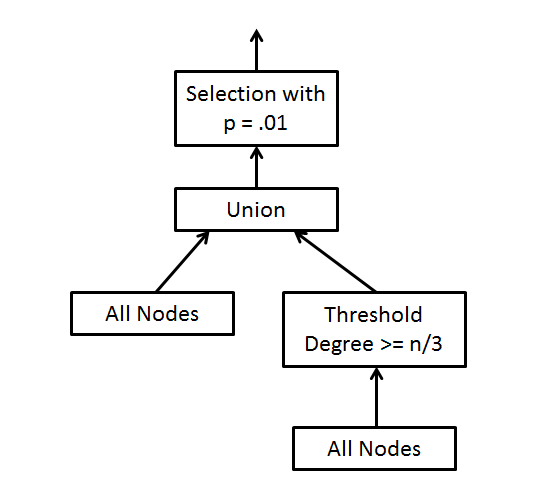
\includegraphics[scale=0.6]{RandomGraphExample}
  \caption{Example Random Graph Generating Parse Tree}
  \label{fig:example}
\end{centering}
\end{figure}


This paper discusses a method using GP to evolve an algorithm that generates a random graph of with a specified nature.  The method proposed uses Koza style GP to evolve a post-ordered parse tree structure that will represent the algorithm. Most random-graph generating algorithms repeat a node adding phase $n$ times to create a random graph of size $n$. Our algorithm takes advantage of this repetitive nature of random-graph algorithms in such a way that it only evolves the method for adding a node and its connections. In this phase, the parse tree decides which nodes will be adjacent to the new node.

There are two proposed methods that this decision process can be done. One method is for each new node, the algorithm would iterate over every existing node and the parse tree would determine if a connection would be made between that node and the new node. The second method would be for the parse tree to be evaluated one time and determine the set of nodes to which the new node will be connected.  It was determined that the second method would be the preferred option, as it would be easier to construct some of the pre-existing random graph algorithms such as the Erd\H{o}s-R\'{e}nyi model.

The parse tree will be constructed from a set of operations that will be used as the non-terminal nodes and sets of nodes which will be used as the terminal nodes.  Each of the operations will take in one or more sets of nodes and return a single set of nodes. The set of nodes returned by the root node will be the set of nodes that the newly created node will connect to. The terminal nodes will be sets of node such as a random subset of the current node set, the entire node set or the empty set. An example parse tree can be seen in Figure \ref{fig:example}.

The main nodes that will be used as the non-terminal nodes will be selection nodes. These nodes will take a set of nodes and select a subset of those nodes to return to its parent node. One example is the selection criterion that is used in the Erd\H{o}s-R\'{e}nyi model. Every node has a $p$ percent chance of getting selected.  Other selection operations such as k-tournament, proportional selection and others can also be used if there is some measure of the nodes that they can be selected on. This could be the degree of the node or some other property that can be attributed to that node.  Other nodes that will be included are set operation nodes such as union, intersection, and disjoint.  By including selection operations that are taken from current random graph models we are guaranteed to be able to represent those models in the parse tree structure.

To evaluate these parse trees random graphs will be generated using the method described in the parse tree. The parse trees will be given a fitness value based on how closely the graphs they generate comply with a user defined model. For the experiments that will be constructed, the models will be fairly rudimentary to show a proof of concept. An example of this could be all nodes have an equal or near equal degree and the degree is roughly $\frac{n}{3}$, $n$ being the number of nodes in the graph.  The user can specify the model and the standard deviation away from the model that the random graphs may have. For the fitness function, $k$ graphs at evenly spaced intervals between the min and max graph size of interest will be sampled. The difference at each point will be averaged along with the standard deviation used in a weighted sum to give each parse tree a fitness value.

The GP will be using standard GP operators along with other operators to help with a local search of the parse trees. The standard GP operators include subtree crossover and subtree mutation. The new operator is an alternate mutation operator which randomly selects a node of the parse tree and randomly changes the parameters of the operation contained in that node.



\bibliographystyle{abbrv}
\bibliography{sigproc} 


\end{document}


